\newpage
\section{Implementierung}


Umsetzung der Anforderung X.X "Erkennen des Ziels mit einer Abweichung von einem Meter".
\\Dieser Abschnitt erläutert die Umsetzung der Anforderung X.X. Wie bereits erläutert wird GPS zur Abstandsermittlung des Prototypen verwendet. Das bedeutet, während der Nutzer sich auf das Ziel zubewegt wird der Standort über GPS bestimmt. Bereits in Kapitel X ist die Genauigkeit von GPS Positionen angegeben.  Sie liegt bei x Metern. Um mit dieser Genauigkeit erkennen zu können, ob sich ein Spieler am Ziel befindet wurde ein Radius von 10 Metern um den Zielpunkt gewählt. Nach einigen Praxistests wurde deutlich, dass dieser Radius nicht ausreicht. Die Testkandidaten konnten den Zielpunkt trotz des Radius nicht erreichen. Aus diesem Grund entschied man sich dazu die Genauigkeit am Zielpunkt deutlich zu erhöhen, mit iBeacons. In Kapitel X ist bereits auf RadioButtons eingegangen worden. Eine Unterkategorie bilden von diesen, bilden die iBeacons.

iBeacons

Bei iBeacons handelt es sich um eine neue Technologie zur Abstands bzw. Standortbestimmung von Smartphones welche vom Hersteller Apple stammt. Auf Materieller Ebene betrachtet ist ein iBeacon ein kleines Gerät welches ständig Bluetooth Signale sendet. Die verwendete Technik ist Bluetooth Low Energy (BLE). Das Gerät besteht aus

" einer kleinen Platine mit Bluetooth-Sender und einer Knopfzelle. Beides steckt in einem Kunststoffgehäuse, das in der Größe zwischen einem dicken 2-Euro-Stück und einer PC-Maus rangiert."
http://www.golem.de/news/bluetooth-low-energy-ibeacon-ist-mehr-als-ein-leuchtfeuer-1403-105331-2.html

Übertragen werden mit dem Signal nur eine eindeutige ID sowie drei Zahlen. Vorteil der BLE Technologie ist der geringe Stromverbrauch. Laut Hersteller soll ein iBeacon zwischen sechs und vierundzwanzig Monaten ein Signal senden können. Abhängig ist dies von der Signalstärke und dem Sendeintervall. Mit dem 2,4 GHz Signal werden Reichweiten von bis zu 50 Metern erreicht. Ein Smartphones welches das Signal empfängt kann einen ungefähren Abstand zum iBeacon ermitteln. Verwendet man mehrere iBeacons, kann über Triangulation ein genauer Standort bestimmt werden. Besonders an dieser Standortbestimmung ist, dass sie auch in Gebäuden funktioniert. Hier ist GPS teilweise gar nicht oder nur schlecht empfangbar. Daraus resultieren diverse Anwendungsbereich im folgenden sind ein paar aufgelistet:

\begin{description}
\item[$\bullet$]die Navigation und Präsentation von Informationen im Museum

\item[$\bullet$]das Dirigieren von Bahnfahrern zum richtigen Bahnsteig und Wagen

\item[$\bullet$]Rabattprogramme und Kundenkarten

\item[$\bullet$]Abholbenachrichtigungen für vorbestellte Waren beim Betreten des Ladens

\item[$\bullet$]die Automatisierung von Gebäudefunktionen wie Heizung, Licht und Jalousiestellung

\item[$\bullet$]Hinweise auf die Stadion-Einlasskontrolle mit den kürzesten Wartezeiten

\item[$\bullet$]Live-Umfragen unter Teilnehmern einer Vortragsveranstaltung

\item[$\bullet$]kostenlose Lektüre einer Zeitschrift beim Aufenthalt in einem Café

\item[$\bullet$]Bereitstellung der Tageskarte eines Restaurants auf dem Smartphone

\end{description}

\cite{BeaconGolem}


\begin{figure}
  \centering
    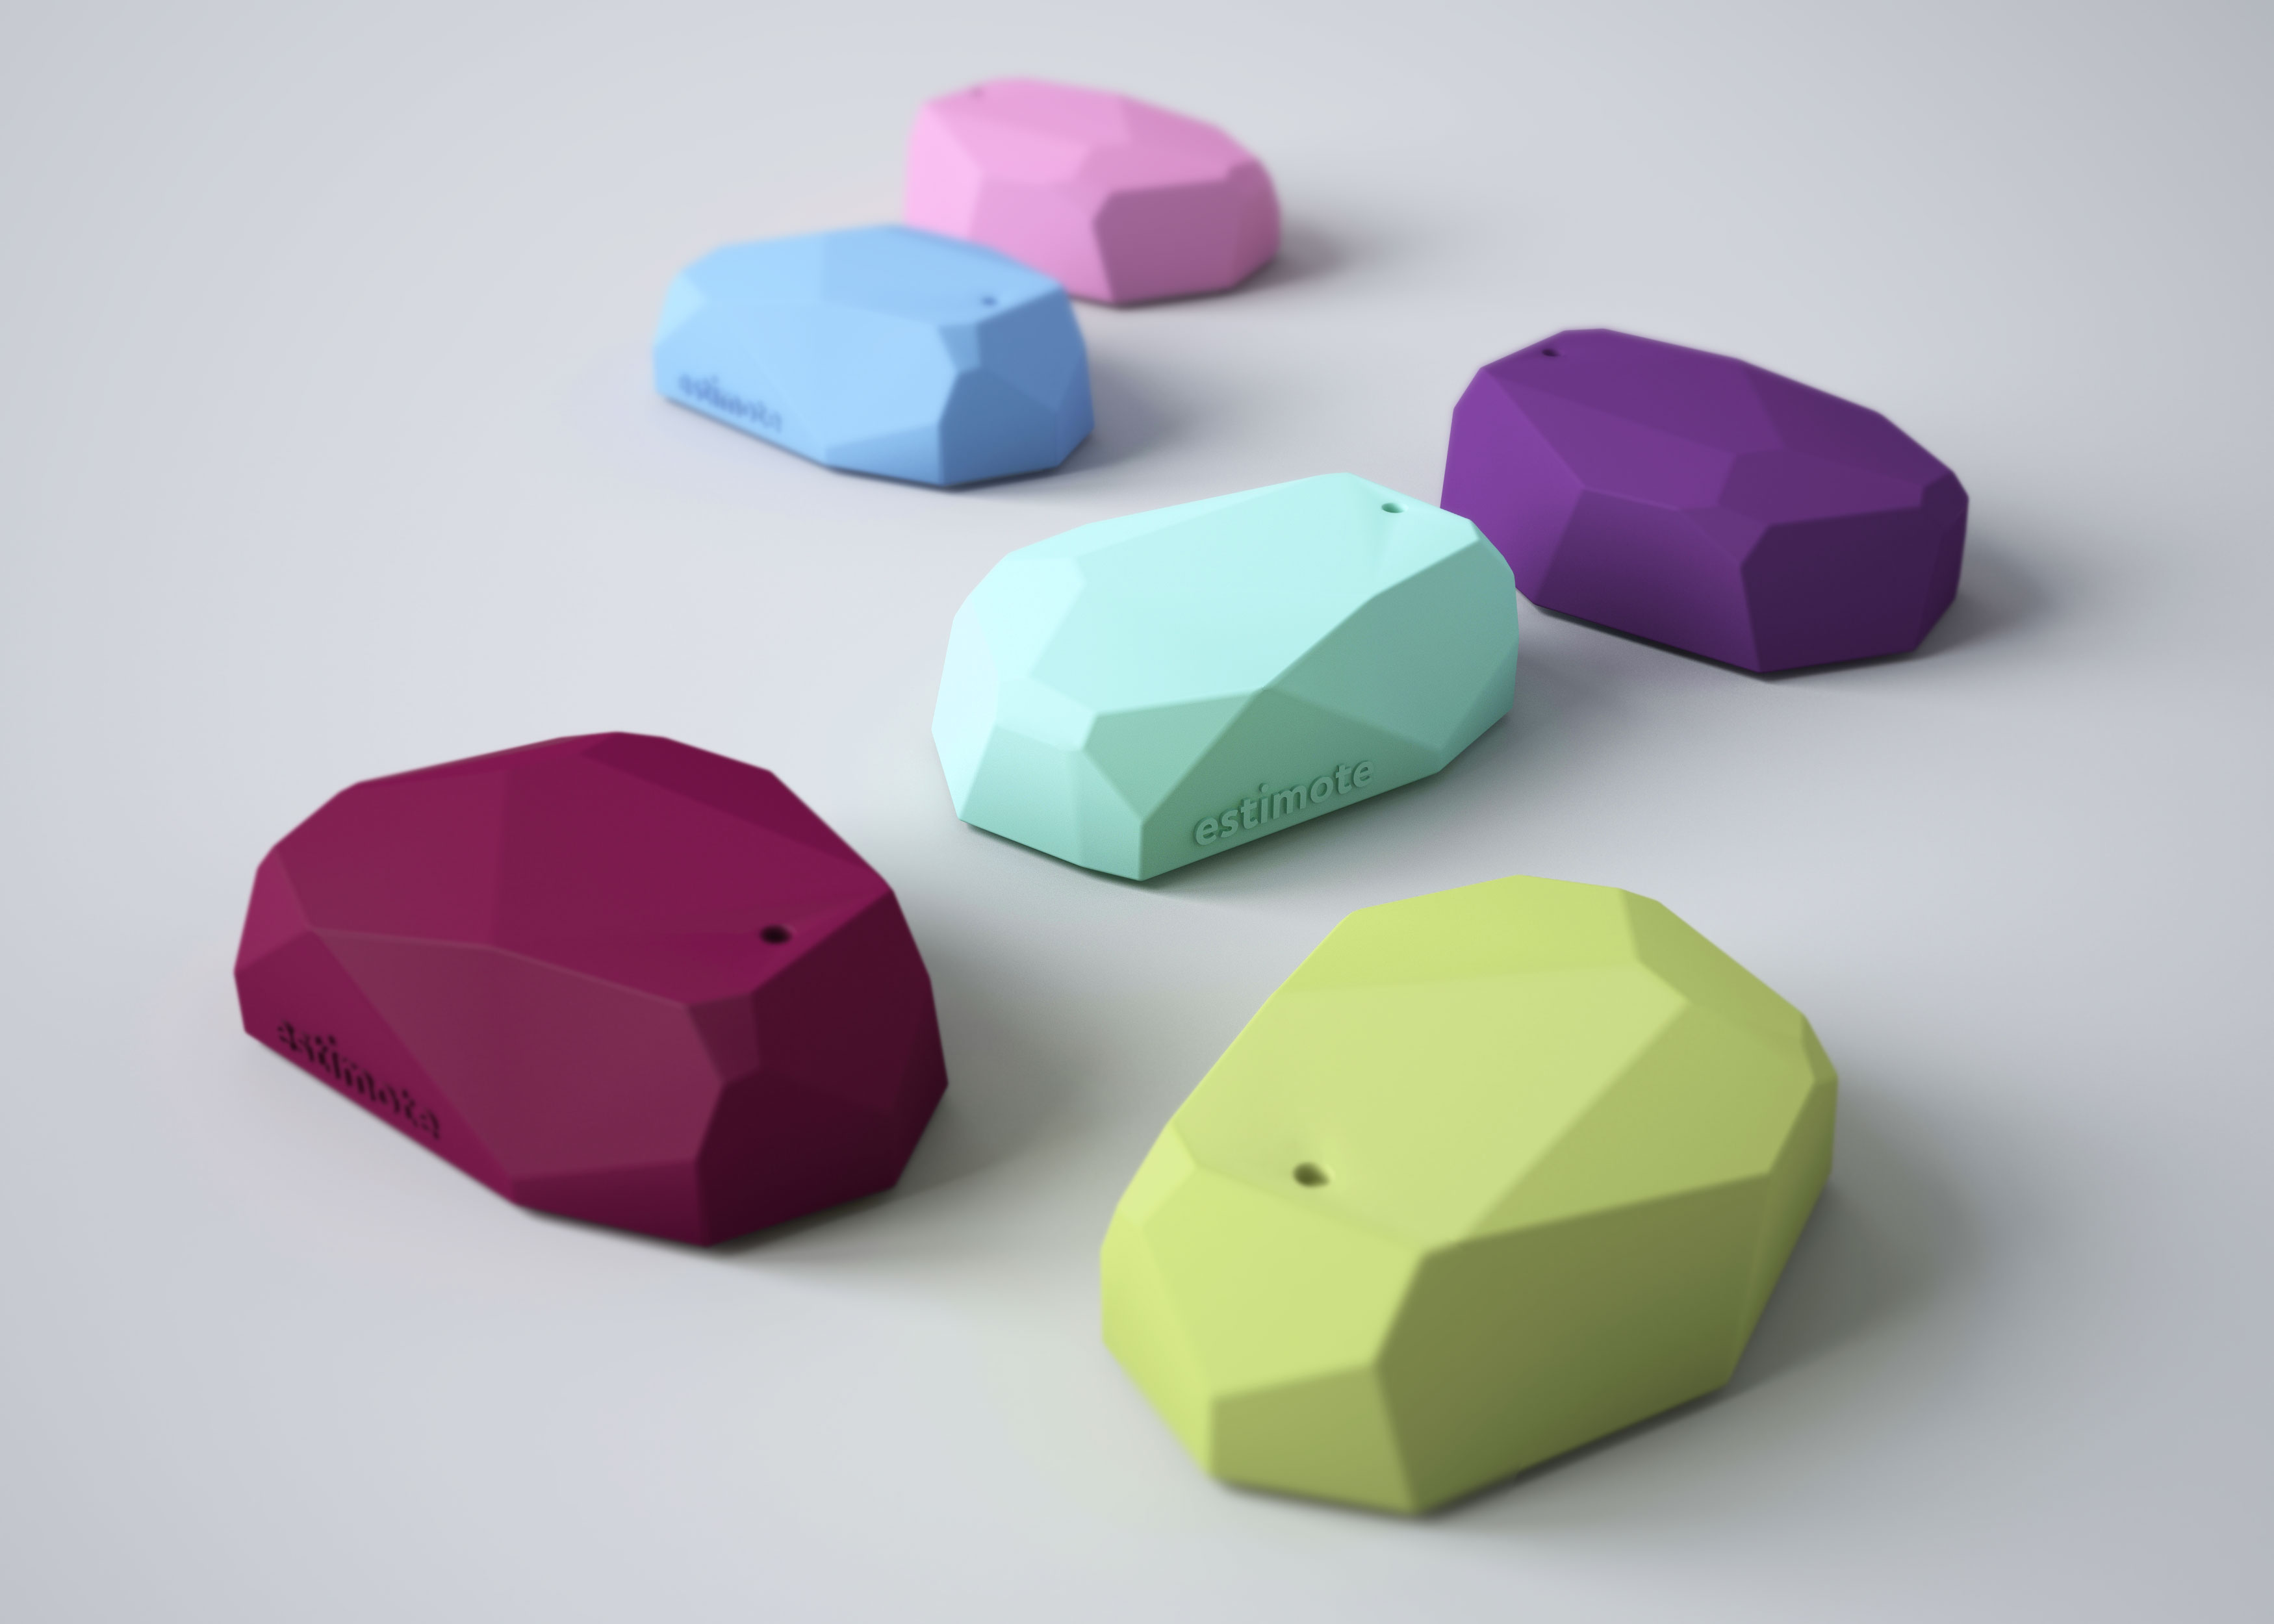
\includegraphics[width=0.5\textwidth]{ref/images/ibeacon.jpg}
   \caption{iBeacons der Firma Estimote}
  \label{fig:iBeacons}
   \cite{iBeacons}
\end{figure}



iBeacons der Firma Estimote

Empfangen werden können die Signale der iBeacons mit Bluetooth 4.0 Empfangsmodulen, welche in den aktuellen Smartphones verbaut sind. Dies funktioniert sowohl mit Apple sowie Android Geräten, was für diese Arbeit von großer Bedeutung ist.


Ziel der Umsetzung in dieser Arbeit ist, dass die definierten Zielpunkte der App mit jeweils einem iBeacon ausgestattet werden. Während der gesamten Ortungsphase läuft im Hintergrund ein iBeacon Scanner. Sobald dieser Scanner den gewünschten iBeacon entdeckt hat wird die Distanz zum Ziel durch den iBeacon bestimmt und nicht per GPS, dadurch wird eine höhere Genauigkeit im Zielgebiet erreicht.

Um dies zu implementieren, muss das Zielpunkt Objekt angepasst werden. Standortobjekte benötigen neben Namen und Positionen noch eine iBeacon ID sowie Major und Minor Werte. 

Mit den neuen Werten sind alle Vorraussetzungen geschaffen um einen iBeacon Scanner zu implementieren. Hierfür wird das Plug-In "Cordova / Phonegap iBeacon plugin" von Peter Metz verwendet. Es ist open Source und kann von Git Hub heruntergeladen werden.

Das Plug-In enthält Schnittstellen und Funktionen zum finden von iBeacons. Hierbei werden zwei unterschiedliche Funktionalitäten geboten.


1. Monitoring von iBeacons
Beim Monitoring wird ständig überprüft ob das Smartphone welches das Plug-In nutzt in einen Bereich eintritt, indem ein iBeacon Signale sendet. Ebenfalls wird überprüft ob das Smartphone den Bereich verlässt. Diese Funktion wird in dieser Arbeit genutzt um dem User anzuzeigen, dass bei Eintritt in eine iBeacon Zone nicht mehr GPS genutzt wird, sondern die Abstandsbestimmung mit Hilfe des iBeacons erfolgt.

2. Ranging von iBeacons
Während Monitoring nur den Aus- bzw. Einritt in eine Zone überprüft, ermittelt das iBeacon Ranging alle in der nähe befindlichen iBeacons und gibt eine ungefähre Distanz zu diesen an. Diese Funktionalität wird genutzt um die Distanz zum Zielort in der App darzustellen.\cite{MonitorRange}




Im folgenden wird die Umsetzung anhand von Quellcode Beispielen erläutert:

Installation
Damit das Plug-In genutzt werden kann, muss es erst über die Console des Betreibssystem installiert werden.

Hierfür navigiert man in der Console zum Hauptordner der App. Dort führt man den Befehl:

\begin{lstlisting}
cordova plugin add https://github.com/petermetz/cordova-plugin-ibeacon.git
\end{lstlisting} 


aus. Draufhin erfolgt die Automatische Installation im Ordner "plugin" der App und es kann auf die Schnittstellen zugegriffen werden.

Der allgemeine Ablauf besteht aus mehreren Schritten:
\begin{enumerate}
\item Schritt Anlegen eines Arrays mit iBeacon Informationen
\item Schritt Hauptfunktion mit for-Schleife aufrufen
\item Schritt Warten auf einen iBeacon in Reichweite
\item Schritt Gefundenes iBeacon-Objekt in Variable schreiben
\item Schritt Daten aus Objekt auslesen und anzeigen
\end{enumerate}



\underline{TODO: An dieser Stelle wird mit Code-Listings die Umsetzung dieser Schritte }\\
\underline{detailliert erläutert werden.}